\section{Implementation}

    \subsection{Admissible meshes}
    \label{sec_mesh}
        
        The sequence of admissible meshes in the HHO method satisfies :

        \begin{defbox}{Admsissible mesh sequences}
            An amdissible mesh sequence for the HHO method is a partition of the volume in \textbf{convex} polyhedra, with an arbitrary number of vertices, such that their faces are \textbf{planar}.
        \end{defbox}

    \subsection{Polynomial Basis}
        
        Insetad of continuous polynomials over $\Mesh$, the displacement field is a discontinuous polynomial, whose set is denoted as $\Pbroken$. The polynomial basis of $\Pbroken$ considered in the HHO method is not the Lagrange polynomial basis, but the monomial basis, which is the assembly of monomials in $\Pbroken$ (\textit{i.e.} the assembly of all $x \mapsto x^{\alpha}$ where $\alpha$ defines the power of the monomial). In addition, the monomial is sclaed with respect to the element in which it acts, so that values taken by the unknown at a given point in $\Omega$ are not influenced by the mesh topolgy.
        \par
        In order to properly define such a basis, we define the following exponents sets :
        \begin{equation}
            \begin{aligned}
                \captize{\alpha}(d, k) =
                \Bigg\{
                    \captize{\alpha}_j(d)
                    \ \ \Bigg\vert \ \ 
                    0 \leq j \leq k
                \Bigg\}
                &&
                \mbox{and}
                &&
                \captize{\alpha}_k(d) =
                \Bigg\{
                    \lighttensori{\alpha} = ({\alpha}\subscript{1}, ..., {\alpha}\subscript{d}) \in \mathbb{N}^d
                    \ \ \Bigg\vert \ \ 
                    \sum_{1 \leq i \leq d} {\alpha}\subscript{i} = k
                \Bigg\}
            \end{aligned}
        \end{equation}
        $\captize{\alpha}_k(d)$ and $\captize{\alpha}(d,k)$ define exponents vectors sets that entirely define the size $N_d^k$ of the polynomial basis to be used such that :
        \begin{equation}
            N_d^k =
            \begin{pmatrix}
                k-d \\ k
            \end{pmatrix}
        \end{equation}
        Let $D \subset \mathbb{R}^d$ a domain with volume $v_D \in \mathbb{R}$, and center of mass $\lighttensori{x}\subscript{D} \in \mathbb{R}^d$.
        The scaled monomial basis $\mathcal{B}_{\mathcal{M}}^k(D, \mathbb{R})$ of size $N_d^k$ in $\mathbb{P}^k(D,\mathbb{R})$ then defines as :
        \begin{equation}
            \mathcal{B}_{\mathcal{M}}^k(D, \mathbb{R}) =
            \Bigg\{
                \tensoro{\theta}\subscript{m} : 
                \lighttensori{x} \mapsto
                \prod_{1 \leq i \leq d}
                {\left(
                    \frac{{x}\subscript{i} - {x}\subscript{i} \subscript{\Domain}}{{v}_{\Domain}}
                \right)}^{{\alpha}\subscript{i}}
                \ \ \Bigg\vert \ \ 
                \lighttensori{\alpha} = ({\alpha}\subscript{1}, ..., {\alpha}\subscript{d}) \in \captize{\alpha}(d,k)
            \Bigg\}
        \end{equation}
        Such a polynomial basis is useful to define polynomials on either cells and faces, since it is directly dependent on the dimension $d$ of the domain $D$.
        Hence, any scalar function $\tensoro{v} \in \mathbb{P}^k(D,\mathbb{R})$ writes as a linear combination of coordinates in $\mathcal{B}_{\mathcal{M}}^k(D, \mathbb{R})$, such that :
        \begin{equation}
            \tensoro{v}
            =
            \sum_{1 \leq m \leq N_d^k} v_m \cdot \tensoro{\theta}\subscript{m}
            =
            \mathbbl{v} \cdot {\mathbbl{b}}\subsupscript{D}{k}
            =
            \mathbbl{v}\supscript{t} \times {\mathbbl{b}}\subsupscript{D}{k}
            \mbox{ with }
            \mathbbl{v} =
            \begin{pmatrix}
                \begin{aligned}
                    v_1
                    \\
                    \vdots
                    \\
                    v_{N_d^k}
                \end{aligned}
            \end{pmatrix}
            \mbox{ and }
            {\mathbbl{b}}\subsupscript{D}{k} =
            \begin{pmatrix}
                \begin{aligned}
                    \tensoro{\theta}\subscript{1}
                    \\
                    \vdots
                    \\
                    \tensoro{\theta}\subscript{N_d^k}
                \end{aligned}
            \end{pmatrix}
        \end{equation}
        where $(v_m)\subscript{1 \leq m \leq N_d^k}$ are the coordinates of $\tensoro{v}$ in $\mathcal{B}_{\mathcal{M}}^k(D, \mathbb{R})$.
        \newline
        With same notations, any vector-valued function $\tensori{v} \in \mathbb{P}^k(D,\mathbb{R}^d)$ writes as :
        \begin{equation}
            \begin{aligned}
                \tensori{v}
                =
                \begin{pmatrix}
                    \begin{aligned}
                        \sum_{1 \leq m \leq N_d^k} {v_0}\subscript{m} \cdot \tensoro{\theta}\subscript{m}
                        \\
                        \vdots
                        \\
                        \sum_{1 \leq m \leq N_d^k} {v_d}\subscript{m} \cdot \tensoro{\theta}\subscript{m}
                    \end{aligned}
                \end{pmatrix}
                =
                \tensori{\mathbbl{v}}\supscript{t} \times \tensori{\mathbbl{b}}\subsupscript{D}{k}
                & \mbox{ with }
                \tensori{\mathbbl{b}}\subsupscript{D}{k} =
                \begin{pmatrix}
                    \begin{aligned}
                        {\mathbbl{b}}\subsupscript{D}{k}
                        \\
                        \vdots
                        \\
                        {\mathbbl{b}}\subsupscript{D}{k}
                    \end{aligned}
                \end{pmatrix}
                \mbox{ and }
                \tensori{\mathbbl{v}} =
                \begin{pmatrix}
                    \begin{aligned}
                        \mathbbl{v}\subscript{1}
                        \\
                        \vdots
                        \\
                        \mathbbl{v}\subscript{d}
                    \end{aligned}
                \end{pmatrix}
            \end{aligned}
        \end{equation}
        \begin{exemplebox}{Scaled monomial basis of order $2$ in a cell $T$ and a face $F$}
            Let $F \subset \mathbb{R}$ with volume (or length) $v_F$ and center of mass ${x}\subscript{F}$, and let the polynomial order $k = 2$. The scaled monomial basis on such a domain writes in vectorial notation :
            \begin{equation}
                {\mathbbl{b}}\subsupscript{F}{2}(x) =
                \begin{pmatrix}
                    \begin{aligned}
                        \begin{pmatrix}
                            \displaystyle
                            \frac{x - x_F}{v_F}
                        \end{pmatrix}
                        ^0
                        \\
                        \begin{pmatrix}
                            \displaystyle
                            \frac{x - x_F}{v_F}
                        \end{pmatrix}
                        ^1
                        \\
                        \begin{pmatrix}
                            \displaystyle
                            \frac{x - x_F}{v_F}
                        \end{pmatrix}
                        ^2
                    \end{aligned}
                \end{pmatrix}
                =
                \begin{pmatrix}
                    \begin{aligned}
                        1
                        \\
                        \begin{matrix}
                            \displaystyle
                            \frac{x - x_F}{v_F}
                        \end{matrix}
                        \\
                        \begin{pmatrix}
                            \displaystyle
                            \frac{x - x_F}{v_F}
                        \end{pmatrix}
                        ^2
                    \end{aligned}
                \end{pmatrix}
            \end{equation}
            Let $T \subset \mathbb{R}^2$ with volume (or surface) $v_T$ and center of mass $\lighttensori{x}\subscript{T}$, and let the polynomial order $k = 2$. The scaled monomial basis on such a domain writes in vectorial notation :
            \begin{equation}
                {\mathbbl{b}}\subsupscript{T}{2}(x,y) = 
                \begin{pmatrix}
                    \begin{aligned}
                        \begin{pmatrix}
                            \displaystyle
                            \frac{x - x_T}{v_T}
                        \end{pmatrix}^0
                        \cdot
                        \begin{pmatrix}
                            \displaystyle
                            \frac{y - y_T}{v_T}
                        \end{pmatrix}^0
                        \\
                        \begin{pmatrix}
                            \displaystyle
                            \frac{x - x_T}{v_T}
                        \end{pmatrix}^0
                        \cdot
                        \begin{pmatrix}
                            \displaystyle
                            \frac{y - y_T}{v_T}
                        \end{pmatrix}^1
                        \\
                        \begin{pmatrix}
                            \displaystyle
                            \frac{x - x_T}{v_T}
                        \end{pmatrix}^1
                        \cdot
                        \begin{pmatrix}
                            \displaystyle
                            \frac{y - y_T}{v_T}
                        \end{pmatrix}^0
                        \\
                        \begin{pmatrix}
                            \displaystyle
                            \frac{x - x_T}{v_T}
                        \end{pmatrix}^0
                        \cdot
                        \begin{pmatrix}
                            \displaystyle
                            \frac{y - y_T}{v_T}
                        \end{pmatrix}^2
                        \\
                        \begin{pmatrix}
                            \displaystyle
                            \frac{x - x_T}{v_T}
                        \end{pmatrix}^1
                        \cdot
                        \begin{pmatrix}
                            \displaystyle
                            \frac{y - y_T}{v_T}
                        \end{pmatrix}^1
                        \\
                        \begin{pmatrix}
                            \displaystyle
                            \frac{x - x_T}{v_T}
                        \end{pmatrix}^2
                        \cdot
                        \begin{pmatrix}
                            \displaystyle
                            \frac{y - y_T}{v_T}
                        \end{pmatrix}^0
                    \end{aligned}
                \end{pmatrix}
                =
                \begin{pmatrix}
                    \begin{aligned}
                        & 1
                        \\
                        & \begin{matrix}
                            \displaystyle
                            \frac{y - y_T}{v_T}
                        \end{matrix}
                        \\
                        & \begin{matrix}
                            \displaystyle
                            \frac{x - x_T}{v_T}
                        \end{matrix}
                        \\
                        & \begin{pmatrix}
                            \displaystyle
                            \frac{y - y_T}{v_T}
                        \end{pmatrix}
                        ^2
                        \\
                        & \begin{pmatrix}
                            \displaystyle
                            \frac{x - x_T}{v_T}
                        \end{pmatrix}
                        \cdot
                        \begin{pmatrix}
                            \displaystyle
                            \frac{y - y_T}{v_T}
                        \end{pmatrix}
                        \\
                        & \begin{pmatrix}
                            \displaystyle
                            \frac{x - x_T}{v_T}
                        \end{pmatrix}
                        ^2
                    \end{aligned}
                \end{pmatrix}
            \end{equation}
        \end{exemplebox}

        Computing the derivative of a polynomial in the sclaed monomial basis amounts to compute the gradient operator $\nabla$ which takes the form of a matrix $\mathbbl{B}\subscript{j} \in \mathbb{R}^{N_d^k \times N_d^k}$ such that, given ${\mathbbl{v}}\supscript{t}$ the coeficients of a function $\tensoro{v}$ in $\mathcal{B}_{\mathcal{M}}^k(D, \mathbb{R})$, the coeficients ${\mathbbl{v}}\subscript{j}$ of the directional derivative $\partial_j \tensoro{v}$ of $\tensoro{v}$ along the $j$-th direction are :
        \begin{equation}
            {\mathbbl{v}}\subscript{,j} = \mathbbl{B}\subscript{j} \times {\mathbbl{v}}
        \end{equation}
        
        \begin{exemplebox}{Continuous gradient operator}
            Let $D \subset \mathbb{R}$. In $\mathcal{B}_{\mathcal{M}}^k(D, \mathbb{R})$, the continuous gradient operator takes the form :
            \begin{equation}
                \begin{aligned}
                    \mathbbl{B}\subscript{1} =
                    \begin{pmatrix}
                        \begin{aligned}
                            0 && 0 && \dots && \dots && 0
                            \\
                            1 && 0 && \dots && \dots && 0
                            \\
                            0 && 2 && \dots && \dots && 0
                            \\
                            0 && 0 && \vdots && \dots && 0
                            \\
                            0 && 0 && \dots && k-1 && 0
                        \end{aligned}
                    \end{pmatrix}
                \end{aligned}
            \end{equation}

            Let $D \subset \mathbb{R}^2$. In $\mathcal{B}_{\mathcal{M}}^2(D, \mathbb{R})$, the continuous gradient operator takes the form :
            \begin{equation}
                \begin{aligned}
                    \mathbbl{B}\subscript{1} =
                    \begin{pmatrix}
                        \begin{aligned}
                            0 && 0 && 0 && 0 && 0 && 0
                            \\
                            0 && 0 && 0 && 0 && 0 && 0
                            \\
                            1 && 0 && 0 && 0 && 0 && 0
                            \\
                            0 && 0 && 0 && 0 && 0 && 0
                            \\
                            0 && 0 && 2 && 0 && 0 && 0
                            \\
                            0 && 0 && 0 && 0 && 0 && 0
                        \end{aligned}
                    \end{pmatrix}
                \end{aligned}
            \end{equation}
            and
            \begin{equation}
                \begin{aligned}
                    \mathbbl{B}\subscript{2} =
                    \begin{pmatrix}
                        \begin{aligned}
                            0 && 0 && 0 && 0 && 0 && 0
                            \\
                            0 && 0 && 0 && 0 && 0 && 0
                            \\
                            0 && 0 && 0 && 0 && 0 && 0
                            \\
                            0 && 0 && 0 && 0 && 0 && 0
                            \\
                            0 && 0 && 0 && 0 && 0 && 0
                            \\
                            0 && 0 && 0 && 0 && 0 && 0
                        \end{aligned}
                    \end{pmatrix}
                \end{aligned}
            \end{equation}
        \end{exemplebox}

    \subsection{Mapping from the cell domain to the face domain}

        \begin{figure}[h!]
            \centering
            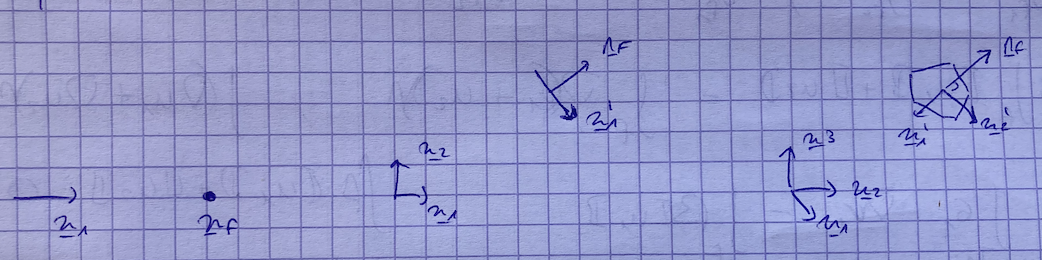
\includegraphics[width=10.cm]{img/mapping_0.png}
            \caption{The considered simplcial mesh for dimensions $d = 1, 2, 3$}
            \label{fig_mapping_0}
        \end{figure}
        Let $T_1$ and $T_2$ two cells linked by a face $F$.
        Let $\lighttensori{x} = (x_1, ..., x_d)$ the coordinates of a point in
        \begin{equation}
            \mathcal{R}^d =
            \{
                \lighttensori{x}\subscript{1}, ..., \lighttensori{x}\subscript{d}
            \}
        \end{equation}
        the canonical (direct orthonormed) reference frame in $\mathbb{R}^d$.
        Let $\lighttensori{n}\subscript{F}$ the normal vector to $F$ in $\mathcal{R}^d$, such that it is outward orientied with respect to the element the observer is in.
        Let 
        \begin{equation}
            \mathcal{R}_F^d =
            \{
                \lighttensori{x}\subsupscript{1}{*}, ..., \lighttensori{x}\subsupscript{d-1}{*}, \lighttensori{x}\subsupscript{d}{*} = {\lighttensori{n}\subscript{F}}/{\lVert \lighttensori{n}\subscript{F} \rVert}
            \}
        \end{equation}
        the rotated orthonormed reference frame in $\mathbb{R}^d$ with respect to $\mathcal{R}^d$ such that the first $d-1$ coordinates in $\mathcal{R}_F^d$ form a direct orthonormed reference frame $\mathcal{R}_F^{d-1}$ in $\mathbb{R}^{d-1}$ :
        \begin{equation}
            \mathcal{R}_F^{d-1} =
            \{
                \lighttensori{x}\subsupscript{1}{*}, ..., \lighttensori{x}\subsupscript{d-1}{*}
            \}
        \end{equation}
        However, $\mathcal{R}_F^d$ is not necesserilly direct since the normal vector to $F$ changes sign depending on the considered cell.

        Let the rotation operator $\lighttensorii{P}\subscript{F}$ from $\mathcal{R}^d$ into $\mathcal{R}_F^d$ :
        \begin{equation}
            \begin{aligned}
                \lighttensori{x}\supscript{*} = \lighttensorii{P}\subscript{F} \lighttensori{x}
                &&
                \forall \lighttensori{x} \in \mathcal{R}^d, \lighttensori{x}\supscript{*} \in \mathcal{R}_F^d
            \end{aligned}
        \end{equation}
        A point with coordinates $\lighttensori{x}\supscript{*} \in \mathcal{R}_F^d$ can then be expressed as a $d-1$ vector $\lighttensori{\kappa} \in \mathcal{R}_F^{d-1}$ and a component $d_F$ (which is the distance of the face to the origin along the direction given by its normal vector) on $\lighttensori{x}\subsupscript{d}{*}$ the normal vector to $F$ :
        \begin{equation}
            \begin{aligned}
                \lighttensori{x}\supscript{*}
                &
                = (\lighttensori{\kappa}, d_F \cdot \lighttensori{x}\subsupscript{d}{*})
                \\
                &
                = (\lighttensorii{P}\subsupscript{F}{\star} \lighttensori{x}, d_F \cdot \lighttensori{x}\subsupscript{d}{*})
            \end{aligned}
        \end{equation}
        Where $\lighttensorii{P}\subsupscript{F}{\star}$ is the restriction of $\lighttensorii{P}\subscript{F}$ to the first $d-1$ rows.
        
        \begin{exemplebox}{Computation of the local reference frame $\mathcal{R}^d_F$ and of $\lighttensorii{P}$}
            \begin{itemize}
                \item
                If $d = 1$, the local reference frame is just a point and the rotation matrix is :
                \begin{equation}
                    \lighttensorii{P}\subscript{F} = \lighttensorii{P}\subsupscript{F}{\star} = 1
                \end{equation}
                \item 
                If $d = 2$, a face is a segment and let $\lighttensori{n}\subscript{1}, \lighttensori{n}\subscript{2}$ its two vertices.
                Let the edge vector $\lighttensori{e} = \lighttensori{n}\subscript{2} - \lighttensori{n}\subscript{1}$.
                the rotation matrix is
                \begin{equation}
                    \lighttensorii{P}\subscript{F} =
                    \begin{pmatrix}
                        \begin{aligned}
                            \frac{e_x}{\lVert \lighttensori{e} \rVert} && \frac{e_y}{\lVert \lighttensori{e} \rVert}
                            \\
                            \frac{e_y}{\lVert \lighttensori{e} \rVert} && -\frac{e_x}{\lVert \lighttensori{e} \rVert}
                        \end{aligned}
                    \end{pmatrix}
                    \mbox{ and }
                    \lighttensorii{P}\subsupscript{F}{\star} =
                    \begin{pmatrix}
                        \begin{aligned}
                            \frac{e_x}{\lVert \lighttensori{e} \rVert} && \frac{e_y}{\lVert \lighttensori{e} \rVert}
                        \end{aligned}
                    \end{pmatrix}
                \end{equation}
                \item
                If $d = 3$, a face is at least a triangle aand at most a polygon, and let $\lighttensori{n}\subscript{1}, \lighttensori{n}\subscript{2}, \lighttensori{n}\subscript{3}, $ three vertices.
                Let the edge vectors $\lighttensori{e}\subscript{1} = \lighttensori{n}\subscript{2} - \lighttensori{n}\subscript{1}$ and $\lighttensori{e}\subscript{t} = \lighttensori{n}\subscript{3} - \lighttensori{n}\subscript{1}$.
                Let $\lighttensori{e}\subscript{3} = \lighttensori{e}\subscript{1} \wedge \lighttensori{e}\subscript{t}$ and $\lighttensori{e}\subscript{2} = \lighttensori{e}\subscript{1} \wedge \lighttensori{e}\subscript{3}$. The rotation matrix is
                \begin{equation}
                    \lighttensorii{P}\subscript{F} =
                    \begin{pmatrix}
                        \begin{aligned}
                            \frac{e_{1x}}{\lVert \lighttensori{e}\subscript{1} \rVert}
                            &&
                            \frac{e_{1y}}{\lVert \lighttensori{e}\subscript{1} \rVert}
                            &&
                            \frac{e_{1z}}{\lVert \lighttensori{e}\subscript{1} \rVert}
                            \\
                            \frac{e_{2x}}{\lVert \lighttensori{e}\subscript{2} \rVert}
                            &&
                            \frac{e_{2y}}{\lVert \lighttensori{e}\subscript{2} \rVert}
                            &&
                            \frac{e_{2z}}{\lVert \lighttensori{e}\subscript{2} \rVert}
                            \\
                            \frac{e_{3x}}{\lVert \lighttensori{e}\subscript{3} \rVert}
                            &&
                            \frac{e_{3y}}{\lVert \lighttensori{e}\subscript{3} \rVert}
                            &&
                            \frac{e_{3z}}{\lVert \lighttensori{e}\subscript{3} \rVert}
                        \end{aligned}
                    \end{pmatrix}
                    \mbox{ and }
                    \lighttensorii{P}\subsupscript{F}{\star} =
                    \begin{pmatrix}
                        \begin{aligned}
                            \frac{e_{1x}}{\lVert \lighttensori{e}\subscript{1} \rVert}
                            &&
                            \frac{e_{1y}}{\lVert \lighttensori{e}\subscript{1} \rVert}
                            &&
                            \frac{e_{1z}}{\lVert \lighttensori{e}\subscript{1} \rVert}
                            \\
                            \frac{e_{2x}}{\lVert \lighttensori{e}\subscript{2} \rVert}
                            &&
                            \frac{e_{2y}}{\lVert \lighttensori{e}\subscript{2} \rVert}
                            &&
                            \frac{e_{2z}}{\lVert \lighttensori{e}\subscript{2} \rVert}
                        \end{aligned}
                    \end{pmatrix}
                \end{equation}
            \end{itemize}
        \end{exemplebox}

        Inversely, a point $P$ with coordinates $\lighttensori{\kappa}\subscript{P}$ in a face (\textit{i.e.} in the $d-1$ domain) can be expressed in $\mathcal{R}^d$ such that $\lighttensori{x}\subscript{P} = (\lighttensorii{P}\subsupscript{F}{-1} \lighttensori{\kappa}\subscript{P}, h_F \cdot \lighttensori{n}\subscript{F} / \lVert \lighttensori{n}\subscript{F} \rVert)$.

        \paragraph{Quadrature points in a face}
        Computing quadrature points in a face $F \subset \mathbb{R}^{d-1}$ amounts to map it onto the canonical reference frame in $\mathbb{R}^{d-1}$, and apply a known quadrature rule (\textit{i.e.} Gauss quadrature rule) using the barycentric coordinates of the face vertices. Since cell unknowns with support in $\mathbb{R}^d$ are also evalutaed on faces, Quadrature points in faces need be expressed in  $\mathcal{R}^d$, and denoting $\lighttensori{\kappa}\subscript{Q} \in \mathbb{R}^{d-1}$ a quadrature point in $F$, its coordinates in $\mathbb{R}^d$ are $\lighttensori{x}\subscript{Q} = (\lighttensori{\kappa}\subscript{Q}, h_F \cdot \lighttensori{n}\subscript{F}/ \lVert \lighttensori{n}\subscript{F}/ \rVert)$


        Hence, computing quadrature points in a face amounts to map it onto the canonical reference frame in $\mathbb{R}^{d-1}$, and apply a known quadrature rule (\textit{i.e.} Gauss quadrature rule) through barycentric coordinates.
        Let 

        \begin{figure}[h!]
            \centering
            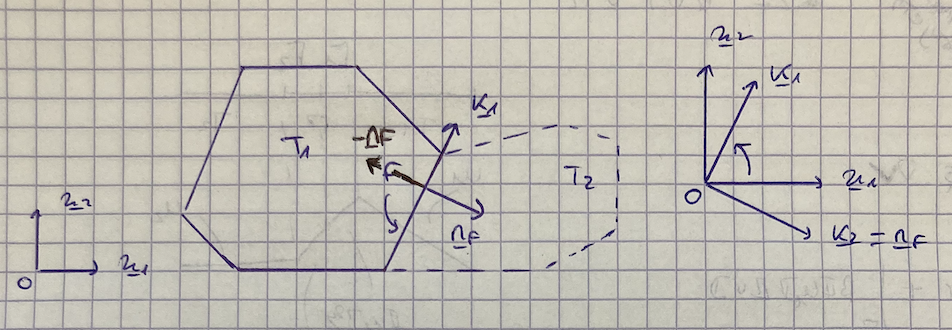
\includegraphics[width=10.cm]{img/geometry_0.png}
            \caption{The considered simplcial mesh for dimensions $d = 1, 2, 3$}
            \label{fig_geometry_0}
        \end{figure}
        \begin{figure}[h!]
            \centering
            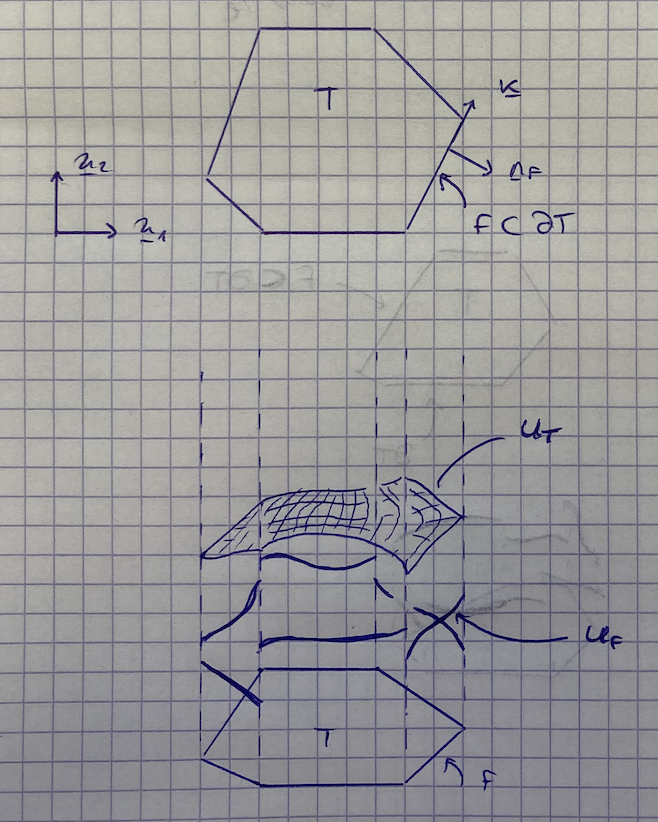
\includegraphics[width=10.cm]{img/geometry_1.png}
            \caption{The considered simplcial mesh for dimensions $d = 1, 2, 3$}
            \label{fig_geometry_1}
        \end{figure}

    \subsection{Integration on polyhedral elements}

        As mentioned in \ref{sec_mesh}, admissible meshes for the HHO method enlarges to any collection of polyhedra with planar faces. However, quadrature rules allow to compute integrals of functions over simplcial domains, such as tetrahedra or hexahedra. In order to compute integrals over polyhedral elements, the latter are particioned in simplices, and quadrature points are then the collection of the quadrature points for simplicies. This amounts to find the center of mass for any polyhedral domain, and then partition it with tetrahedra linking the center of mass to faces.

        \begin{figure}[h!]
            \centering
            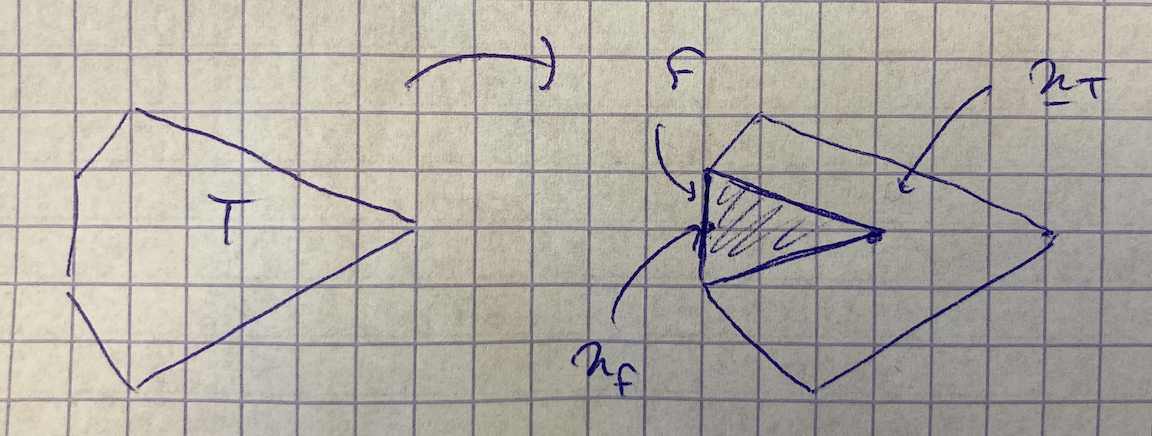
\includegraphics[width=10.cm]{img/partition_0.png}
            \caption{The considered simplcial mesh for dimensions $d = 1, 2, 3$}
            \label{fig_partition_0}
        \end{figure}
        \begin{figure}[h!]
            \centering
            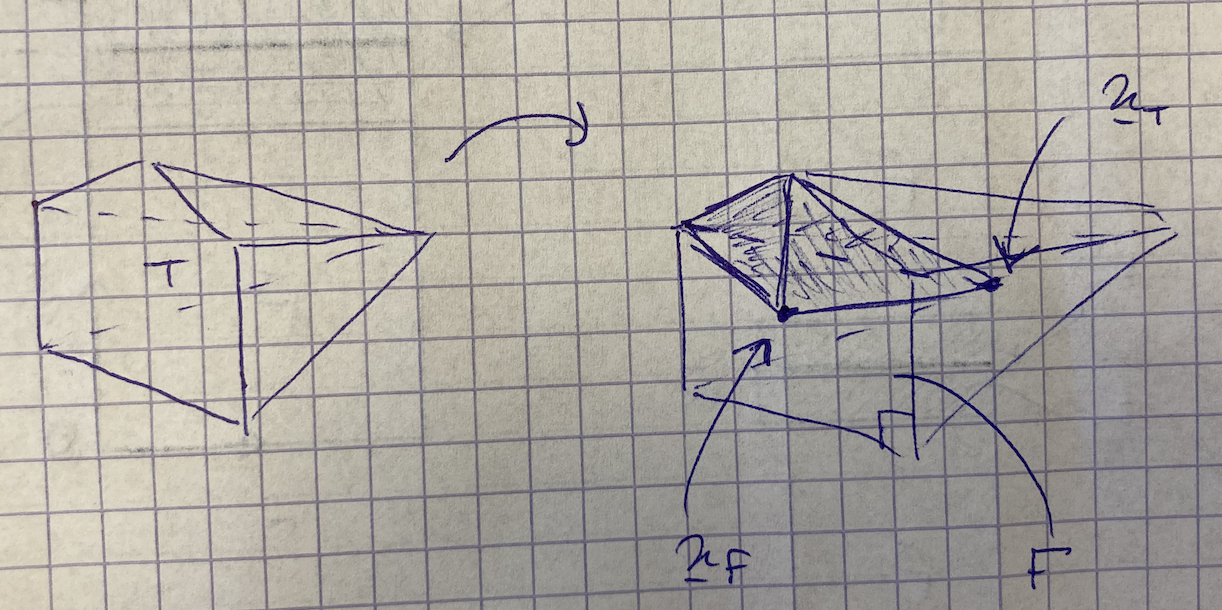
\includegraphics[width=10.cm]{img/partition_1.png}
            \caption{The considered simplcial mesh for dimensions $d = 1, 2, 3$}
            \label{fig_partition_1}
        \end{figure}

        Let $\mathcal{Q}_D^k$ a quadrature rule of order $k_Q$ on a any polhyderal domain $D$ : the $N_Q$ quadrature points are denoted as $(\lighttensori{x}\subscript{{Q}}\subscript{i})\subscript{1 \leq i \leq N_Q}$, and the $N_Q$ quadrature weights are denoted as $({w}\subscript{{Q}}\subscript{i})\subscript{1 \leq i \leq N_Q}$

        Hence, let $\tensori{v}$ a vectorial function in $D \subset \mathbb{R}^{d}$ :
        \begin{equation}
            \int_D \tensori{v} = \sum_{1 \leq i \leq N_Q} w\subscript{{Q}}\subscript{i} \tensori{v}(\lighttensori{x}\subscript{Q}\subscript{i})
        \end{equation}
        Let $\tensori{u}$ (resp. $\tensori{v}$) in $\mathbb{P}^k(D,\mathbb{R}^d)$ (resp. in $\mathbb{P}^l(D,\mathbb{R}^d)$) with coeficients $\tensori{\bbupsilon}$ (resp. $\tensori{\bbnu}$) in $\mathcal{B}_{\mathcal{M}}^k(D, \mathbb{R}^d)$ (resp. in $\mathcal{B}_{\mathcal{M}}^l(D, \mathbb{R}^d)$).
        Let $\tensori{\bbtheta} = \lighttensori{\mathbbl{b}}\subsupscript{D}{k}$ the vectorial representation of $\mathcal{B}_{\mathcal{M}}^k(D, \mathbb{R}^d)$, and $\tensori{\bbomega} = \lighttensori{\mathbbl{b}}\subsupscript{D}{l}$ that of $\mathcal{B}_{\mathcal{M}}^l(D, \mathbb{R}^d)$, such that $\tensori{u} = \tensori{\bbupsilon} \cdot \tensori{\bbtheta}$ and $\tensori{v} = \tensori{\bbnu} \cdot \tensori{\bbomega}$.
        
        Let $\mathcal{Q}_D^{k_Q}$ a quadrature rule of order $k_Q = \max\{k^2,l^2\}$ over $D$.
        One has :
        \begin{equation}
            \begin{aligned}
                \int_D \tensori{u}
                &
                =
                \sum_{1 \leq i \leq N_Q}
                \sum_{1 \leq m \leq N_d^k}
                w\subscript{{Q}}\subscript{i}
                \cdot
                \lighttensori{u}\subscript{m} \tensori{\theta}\subscript{m}(\lighttensori{x}\subscript{Q}\subscript{i})
                \\
                & =
                \sum_{1 \leq i \leq N_Q}
                w\subscript{{Q}}\subscript{i}
                \cdot
                \lighttensori{\bbupsilon}\supscript{t}
                \times
                \tensori{\bbtheta}(\lighttensori{x}\subscript{Q}\subscript{i})
            \end{aligned}
        \end{equation}
        And the product inside the integral sign takes the discrete formulation :
        \begin{equation}
            \begin{aligned}
                \int_D \tensoro{u} \cdot \tensoro{v}
                & =
                \sum_{1 \leq i \leq N_Q}
                w\subscript{{Q}}\subscript{i}
                \cdot
                \tensoro{u}(\lighttensori{x}\subscript{Q}\subscript{i})
                \cdot
                \tensoro{v}(\lighttensori{x}\subscript{Q}\subscript{i})
                \\
                & =
                \sum_{1 \leq i \leq N_Q}
                \sum_{1 \leq m \leq N_d^k}
                \sum_{1 \leq n \leq N_d^l}
                w\subscript{{Q}}\subscript{i}
                \cdot
                \lighttensoro{u}\subscript{m} \tensoro{\theta}\subscript{m}(\lighttensori{x}\subscript{Q}\subscript{i})
                \cdot
                \lighttensoro{v}\subscript{n} \tensoro{\omega}\subscript{n}(\lighttensori{x}\subscript{Q}\subscript{i})
                \\
                & =
                \sum_{1 \leq i \leq N_Q}
                w\subscript{{Q}}\subscript{i}
                \cdot
                \lighttensoro{\bbupsilon}\supscript{t}
                \times
                \tensoro{\bbtheta}(\lighttensori{x}\subscript{Q}\subscript{i})
                \times
                \tensoro{\bbomega}\supscript{t}(\lighttensori{x}\subscript{Q}\subscript{i})
                \times
                \lighttensoro{\bbnu}
                \\
                & =
                \sum_{1 \leq i \leq N_Q}
                w\subscript{{Q}}\subscript{i}
                \cdot
                \lighttensoro{\bbupsilon}\supscript{t}
                \times
                {\mathbbl{M}}\subsupscript{D}{m}(\lighttensori{x}\subscript{Q}\subscript{i})
                \times
                \lighttensoro{\bbnu}
            \end{aligned}
        \end{equation}
        Where ${\mathbbl{M}}\subsupscript{D}{m}$ is the mass matrix formed by the product $\tensori{\bbtheta} \times \tensori{\bbomega}\supscript{t}$

        Let now consider the advection product inside the integral sign :
        \begin{equation}
            \begin{aligned}
                \int_D \partial_j \tensoro{u} \cdot \tensoro{v}
                & =
                \sum_{1 \leq i \leq N_Q}
                w\subscript{{Q}}\subscript{i}
                \cdot
                \partial_j \tensoro{u}(\lighttensori{x}\subscript{Q}\subscript{i})
                \cdot
                \tensoro{v}(\lighttensori{x}\subscript{Q}\subscript{i})
                \\
                & =
                \sum_{1 \leq i \leq N_Q}
                \sum_{1 \leq m \leq N_d^k}
                \sum_{1 \leq n \leq N_d^l}
                w\subscript{{Q}}\subscript{i}
                \cdot
                \lighttensoro{u}\subscript{m} \partial_j\tensoro{\theta}\subscript{m}(\lighttensori{x}\subscript{Q}\subscript{i})
                \cdot
                \lighttensoro{v}\subscript{n} \tensoro{\omega}\subscript{n}(\lighttensori{x}\subscript{Q}\subscript{i})
                \\
                & =
                \sum_{1 \leq i \leq N_Q}
                w\subscript{{Q}}\subscript{i}
                \cdot
                \lighttensoro{\bbupsilon}\supscript{t}
                \times
                \mathbbl{B}\subscript{j}
                \times
                \tensoro{\bbtheta}(\lighttensori{x}\subscript{Q}\subscript{i})
                \times
                \tensoro{\bbomega}\supscript{t}(\lighttensori{x}\subscript{Q}\subscript{i})
                \times
                \lighttensoro{\bbnu}
                \\
                & =
                \sum_{1 \leq i \leq N_Q}
                w\subscript{{Q}}\subscript{i}
                \cdot
                \lighttensoro{\bbupsilon}\supscript{t}
                \times
                {\mathbbl{M}\subsupscript{D}{a}}(\lighttensori{x}\subscript{Q}\subscript{i})
                \times
                \lighttensoro{\bbnu}
            \end{aligned}
        \end{equation}

        With the advection matrix $\mathbbl{M}\subsupscript{D}{a} = \mathbbl{B}\subscript{j}
        \times
        \tensoro{\bbtheta}(\lighttensori{x}\subscript{Q}\subscript{i})
        \times
        \tensoro{\bbomega}\supscript{t}(\lighttensori{x}\subscript{Q}\subscript{i})$

    \subsection{Polynomial order and spatial dimension in an element}

        Let $\tensori{u}\subscript{\bm{T}} \in \mathbb{P}^l(T, \mathbb{R}^d)$ the unknown in the cell $T \subset \mathbb{R}^d$, and $\tensori{u}\subscript{\bm{F}} \in \mathbb{P}^k(F, \mathbb{R}^d)$ that in the face $F \subset \mathbb{R}^{d-1}$.
        Let $\mathcal{B}_{\mathcal{M}}^l(T, \mathbb{R})$ (resp. $\mathcal{B}_{\mathcal{M}}^k(F, \mathbb{R})$) the polynomial basis in $T$ (resp. $F$), with vectorial notations $\bbtheta = \mathbbl{b}_T^l$ (resp. $\bbomega = \mathbbl{b}_F^k$)
        \newline
        Let $\tensori{\mathbbl{u}}\subscript{T}$ the unknown vector in $T$, and $\tensori{\mathbbl{u}}\subscript{F}$ that in $F$, such that :
        \begin{equation}
            \tensori{u}\subscript{T}(\lighttensori{x}) = \tensori{\mathbbl{u}}\subsupscript{T}{t} \times \tensori{\bbtheta}(\lighttensori{x})
            \mbox{ and }
            \tensori{u}\subscript{F}(\lighttensori{\kappa}) = \tensori{\mathbbl{u}}\subsupscript{F}{t} \times \tensori{\bbomega}(\lighttensori{\kappa})
        \end{equation}
    
    \subsection{Computation of the reconstructed gradient}
        
        The reconstructed gradient solves :
        \begin{equation}
            \label{eq_grad_rec_0}
            \begin{aligned}
                & \int_T \tensorii{\tau} : \tensorii{G}\subscript{\bm{T}} = \int_T \tensorii{\tau} : \nabla \tensori{u}\subscript{\bm{T}} + \sum_{F \in \mathcal{F}(T)} \int_{F} \tensorii{\tau} \lighttensori{n}\subscript{F} \cdot (\tensori{u}\subscript{\bm{F}} - \tensori{u}\subscript{\bm{T}} \vert_F)
                &&
                \forall \tensorii{\tau}
            \end{aligned}
        \end{equation}
        Let $\mathcal{Q}_F^k$ a quadrature rule of order $k_Q = \max{2l,2k}$ for each face, and $\mathcal{Q}_T^l$ the quadrature of order $k_Q$ in the cell. Let $\lighttensori{x}\subscript{Q_F}$ a quafdarture point in the face $F$ and $\lighttensori{x}\subscript{Q_T}$ one in the cell $T$. Then, the projection of \eqref{eq_grad_rec_0} onto each component reads :
        \begin{equation}
            \begin{aligned}
                &
                \sum_{\lighttensori{x}\subscript{Q_T}} \tensoro{\tau}\subscript{ij} : \tensoro{G}\subscript{\bm{T}}\subscript{ij}
                =
                \sum_{\lighttensori{x}\subscript{Q_T}} \tensoro{\tau}\subscript{ij} : \tensoro{u}\subscript{\bm{T}}\subscript{i,j}
                +
                \sum_{F \in \mathcal{F}(T)} \sum_{\lighttensori{x}\subscript{Q_F}} \tensoro{\tau}\subscript{ij} n_{Fj} \cdot (\tensoro{u}\subscript{\bm{F}}\subscript{i}
                -
                \tensoro{u}\subscript{\bm{T}}\subscript{i} \vert_F)
                &&
                \forall \tensoro{\tau}\subscript{ij}
            \end{aligned}
        \end{equation}
        Which gives, in matricial formulation :
        \begin{equation}
            \begin{aligned}
                \sum_{\lighttensori{x}\subscript{Q_T}} \bbtau\subsupscript{ij}{t} \times {\mathbbl{M}}\subsupscript{T}{m}(\lighttensori{x}\subscript{Q_T}) \times \mathbbl{G}\subscript{{T}}\subscript{ij}
                &
                =
                \sum_{\lighttensori{x}\subscript{Q_T}} \bbtau\subsupscript{ij}{t} \times {\mathbbl{M}}\subsupscript{Tj}{a}(T)(\lighttensori{x}\subscript{Q_T}) \times \mathbbl{u}\subscript{{T}}\subscript{i}
                \\
                &
                +
                \sum_{F \in \mathcal{F}(T)} \sum_{\lighttensori{x}\subscript{Q_F}}
                \big(
                    \bbtau\subsupscript{ij}{t} n_{Fj} \times {\mathbbl{M}}\subsupscript{F}{h}(\lighttensori{x}\subscript{Q_F}) \times \mathbbl{u}\subscript{{F}}\subscript{i}
                    -
                    \bbtau\subsupscript{ij}{t} n_{Fj} \times {\mathbbl{M}}\subsupscript{F}{m}(\lighttensori{x}\subscript{Q_F}) \times \mathbbl{u}\subscript{{T}}\subscript{i}
                \big)
            \end{aligned}
        \end{equation}
        Defining the following integration matrices in the cell :
        \begin{equation}
            \begin{aligned}
                & {\mathbbl{M}}\subsupscript{T}{m}(\lighttensori{x}\subscript{Q_T}) = \bbtheta(\lighttensori{x}\subscript{Q_T}) \times \bbtheta^t(\lighttensori{x}\subscript{Q_T})
                &&
                \mbox{and}
                &&
                {\mathbbl{M}}\subsupscript{T}{m}(T) =
                \sum_{\lighttensori{x}\subscript{Q_T}}
                {\mathbbl{M}}\subsupscript{T}{m}(\lighttensori{x}\subscript{Q_T})
                \\
                & {\mathbbl{M}}\subsupscript{Tj}{a}(\lighttensori{x}\subscript{Q_T}) = \bbtheta(\lighttensori{x}\subscript{Q_T}) \times (\mathbbl{B}_j \times \bbtheta)^t(\lighttensori{x}\subscript{Q_T})
                &&
                \mbox{and}
                &&
                {\mathbbl{M}}\subsupscript{Tj}{a}(T) =
                \sum_{\lighttensori{x}\subscript{Q_T}}
                {\mathbbl{M}}\subsupscript{Tj}{a}(\lighttensori{x}\subscript{Q_T})
            \end{aligned}
        \end{equation}
        And, for any $F$, the following integration matrices in the $F$ :
        \begin{equation}
            \begin{aligned}
                & {\mathbbl{M}}\subsupscript{F}{h}(\lighttensori{x}\subscript{Q_F}) = \bbtheta(\lighttensori{x}\subscript{Q_F}) \times \bbomega^t(\lighttensorii{P}\subsupscript{F}{\star}\lighttensori{x}\subscript{Q_F})
                &&
                \mbox{and}
                &&
                {\mathbbl{M}}\subsupscript{F}{h}(F) =
                \sum_{\lighttensori{x}\subscript{Q_F}}
                {\mathbbl{M}}\subsupscript{F}{h}(\lighttensori{x}\subscript{Q_F})
                \\
                & {\mathbbl{M}}\subsupscript{F}{m}(\lighttensori{x}\subscript{Q_F}) = \bbtheta(\lighttensori{x}\subscript{Q_F}) \times \bbtheta^t(\lighttensori{x}\subscript{Q_F})
                &&
                \mbox{and}
                &&
                {\mathbbl{M}}\subsupscript{F}{m}(F) =
                \sum_{\lighttensori{x}\subscript{Q_F}}
                {\mathbbl{M}}\subsupscript{F}{m}(\lighttensori{x}\subscript{Q_F})
            \end{aligned}
        \end{equation}
        One has the following matricial expression of \eqref{eq_grad_rec_0} :
        \begin{equation}
            \begin{aligned}
                \bbtau\subsupscript{ij}{t} \times {\mathbbl{M}}\subsupscript{T}{m} \times \mathbbl{G}\subscript{{T}}\subscript{ij}
                =
                \bbtau\subsupscript{ij}{t} \times {\mathbbl{M}}\subsupscript{Tj}{a}(T) \times \mathbbl{u}\subscript{{T}}\subscript{i}
                +
                \sum_{F \in \mathcal{F}(T)} \bbtau\subsupscript{ij}{t} n_{Fj} \times {\mathbbl{M}}\subsupscript{F}{h} \times \mathbbl{u}\subscript{{F}}\subscript{i}
                -
                \sum_{F \in \mathcal{F}(T)} \bbtau\subsupscript{ij}{t} n_{Fj} \times {\mathbbl{M}}\subsupscript{F}{m} \times \mathbbl{u}\subscript{{T}}\subscript{i}
            \end{aligned}
        \end{equation}
        Since $\tensorii{\tau}$ is arbitrary, the vector $\mathbbl{G}\subscript{{T}}\subscript{ij}$ is entirely defined by the system :
        \begin{equation}
            \begin{aligned}
                {\mathbbl{M}}\subsupscript{T}{m} \times \mathbbl{G}\subscript{{T}}\subscript{ij}
                & =
                {\mathbbl{M}}\subsupscript{Tj}{a}(T) \times \mathbbl{u}\subscript{{T}}\subscript{i}
                +
                \sum_{F \in \mathcal{F}(T)} n_{Fj} {\mathbbl{M}}\subsupscript{F}{h} \times \mathbbl{u}\subscript{{F}}\subscript{i}
                -
                \sum_{F \in \mathcal{F}(T)} n_{Fj} {\mathbbl{M}}\subsupscript{F}{m} \times \mathbbl{u}\subscript{{T}}\subscript{i}
                \\
                & =
                \begin{pmatrix}
                    \begin{aligned}
                        {\mathbbl{M}}\subsupscript{Tj}{a}(T)
                        - ({\mathbbl{M}}\subsupscript{F}{m} n_{F_1j}
                        + \dots
                        + {\mathbbl{M}}\subsupscript{F_{N_{\partial T}}}{m} n_{F_{N_{\partial T}}j})
                        &&
                        {\mathbbl{M}}\subsupscript{F_1}{h}
                        &&
                        \dots
                        &&
                        {\mathbbl{M}}\subsupscript{F_{N_{\partial T}}}{h} n_{F_{N_{\partial T}}j})
                    \end{aligned}
                \end{pmatrix}
                \times
                \mathbbl{u}_i^t
            \end{aligned}
        \end{equation}
        Hence, letting $\mathbbl{B}\subscript{Tj}$ the local gradient operator such that $\mathbbl{G}\subscript{Tij} = \mathbbl{B}\subscript{Tj} \times \mathbbl{u}_i^t$, one has :
        \begin{equation}
            \label{eq_grad_rec_1}
            \mathbbl{B}\subscript{Tj} = 
            ({\mathbbl{M}}\subsupscript{T}{m})\supscript{-1}
            \times
            \begin{pmatrix}
                \begin{aligned}
                    {\mathbbl{M}}\subsupscript{Tj}{a}(T)
                    - ({\mathbbl{M}}\subsupscript{F}{m} n_{F_1j}
                    + \dots
                    + {\mathbbl{M}}\subsupscript{F_{N_{\partial T}}}{m} n_{F_{N_{\partial T}}j})
                    &&
                    {\mathbbl{M}}\subsupscript{F_1}{h} n_{F_1j}
                    &&
                    \dots
                    &&
                    {\mathbbl{M}}\subsupscript{F_{N_{\partial T}}}{h} n_{F_{N_{\partial T}}j}
                \end{aligned}
            \end{pmatrix}
        \end{equation}

        \begin{infobox}{Building the descrete gradient operator for vector-valued fields}
            The descrete gradient operator $\mathbbl{B}\subscript{Tj}$ defined in \eqref{eq_grad_rec_1} is built such that is acts on a scalar field, namely the unknown $\mathbbl{u}_i$. However, considering vector-valued unknowns $\tensori{\mathbbl{u}}$, one needs to build a larger operator with zeros on lines and columns corresponding to directions on which the gradient operator does not act.
            For conciseness, let :
            \begin{equation}
                \begin{aligned}
                    \mathbbl{M}_{Tj} = 
                    ({\mathbbl{M}}\subsupscript{T}{m})\supscript{-1}
                    \times
                    ({\mathbbl{M}}\subsupscript{Tj}{a}(T)
                    - ({\mathbbl{M}}\subsupscript{F}{m} n_{F_1j}
                    + \dots
                    + {\mathbbl{M}}\subsupscript{F_{N_{\partial T}}}{m} n_{F_{N_{\partial T}}j}))
                \end{aligned}
            \end{equation}
            and, for any $F$ :
            \begin{equation}
                \begin{aligned}
                    \mathbbl{M}_F = 
                    ({\mathbbl{M}}\subsupscript{T}{m})\supscript{-1}
                    \times
                    {\mathbbl{M}}\subsupscript{F}{h} n_{Fj}
                \end{aligned}
            \end{equation}
            Then, using the multi-index notation $\mathfrak{i}$ for the indices $i,j$ :
            \begin{equation}
                \begin{aligned}
                    \tensorii{\mathbbl{B}}\subscript{T}
                    =
                    (\mathbbl{B}_{Tij})\subscript{1 \leq i,j \leq d}
                    =
                    (\mathbbl{B}_{T\mathfrak{i}})\subscript{1 \leq \mathfrak{i} \leq d^2}
                \end{aligned}
            \end{equation}
            Such that :
            \begin{equation}
                \begin{aligned}
                    \mathbbl{B}_{T\mathfrak{i}}
                    =
                    \begin{pmatrix}
                        \begin{aligned}
                            \underbrace{
                                \begin{aligned}
                                    0 && \dots && \mathbbl{M}_{Tj} && \dots && 0
                                \end{aligned}
                            }_{d \cdot N_d^l}
                            &&
                            \overbrace{
                                \begin{aligned}
                                    \underbrace{
                                        \begin{aligned}
                                            0 && \dots && \mathbbl{M}_F && \dots && 0
                                        \end{aligned}
                                    }_{d \cdot N_{d-1}^k}
                                    &&
                                    \dots
                                    &&
                                    \underbrace{
                                        \begin{aligned}
                                            0 && \dots && \mathbbl{M}_F && \dots && 0
                                        \end{aligned}
                                    }_{d \cdot N_{d-1}^k}
                                \end{aligned}
                            }^{N_{\partial T} \cdot d \cdot N_{d-1}^k}
                        \end{aligned}
                    \end{pmatrix}
                \end{aligned}
            \end{equation}
        \end{infobox}
    
\section{Resolution}

    \subsection{Static condensation}

        Let $\mathbbl{u}\subsupscript{{T}}{t,m}, \mathbbl{u}\subsupscript{{\partial T}}{t,m}$ the displacement at a given time $t$, and at a given iteration $m$

        Let the residual $\mathbbl{R}^{t,m}$ such that :
        \begin{equation}
            \mathbbl{R}^{t,m}
            =
            \mathbbl{F}^{t,m}
            -
            \mathbbl{B}^{t+\Delta t}
        \end{equation}
        with inner forces $\mathbbl{F}^{t,m} = \mathbbl{F}(\Delta\mathbbl{u}\subsupscript{{T}}{t,m}, \Delta\mathbbl{u}\subsupscript{{\partial T}}{t,m})$ and external forces $\mathbbl{B}^{t+\Delta t}$ evaluated at the time $t+\Delta t$.
        Decomposing on faces and cell :
        \begin{equation}
            \begin{aligned}
                & \mathbbl{R}_{T}^{t,m}
                =
                \mathbbl{F}_{T}^{t,m}
                -
                \mathbbl{B}_{T}^{t+\Delta t}
                \\
                & \mathbbl{R}_{\partial T}^{t,m}
                =
                \mathbbl{F}_{\partial T}^{t,m}
                -
                \mathbbl{B}_{\partial T}^{t+\Delta t}
            \end{aligned}
        \end{equation}
        And linearizing yields :
        \begin{equation}
            \begin{aligned}
                \begin{pmatrix}
                    \begin{aligned}
                        \mathbbl{R}_{T}^{t,m+1}
                        \\
                        \mathbbl{R}_{\partial T}^{t,m+1}
                    \end{aligned}
                \end{pmatrix}
                \approx
                0
                & \iff
                \begin{pmatrix}
                    \begin{aligned}
                        \mathbbl{K}_{T T}^{t,m} && \mathbbl{K}_{T \partial T}^{t,m}
                        \\
                        \mathbbl{K}_{\partial T T}^{t,m} && \mathbbl{K}_{\partial T \partial T}^{t,m}
                    \end{aligned}
                \end{pmatrix}
                \begin{pmatrix}
                    \begin{aligned}
                        \delta \Delta \mathbbl{u}\subsupscript{{T}}{t,m}
                        \\
                        \delta \Delta \mathbbl{u}\subsupscript{{\partial T}}{t,m}
                    \end{aligned}
                \end{pmatrix}
                \approx
                -
                \begin{pmatrix}
                    \begin{aligned}
                        \mathbbl{R}_{T}^{t,m}
                        \\
                        \mathbbl{R}_{\partial T}^{t,m}
                    \end{aligned}
                \end{pmatrix}
            \end{aligned}
        \end{equation}
        Since $\mathbbl{K}_{T T}^{t,m}$ is invertible, one can express $\delta \Delta \mathbbl{u}\subsupscript{{T}}{t,m}$ as a linear function of $\delta \Delta \mathbbl{u}\subsupscript{{\partial T}}{t,m}$:
        \begin{equation}
            {\mathbbl{K}}\subsupscript{c}{t,m}
            \times
            \delta \Delta {\mathbbl{u}}\subsupscript{{\partial T}}{t,m}
            =
            - {\mathbbl{R}}\subsupscript{c}{t,m}
        \end{equation}
        With
        \begin{equation}
            \mathbbl{K}_{c}^{t,m}
            =
            \mathbbl{K}_{\partial T \partial T}^{t,m}
            -
            \mathbbl{K}_{\partial T T}^{t,m}
            (\mathbbl{K}_{T T}^{t,m})\supscript{-1}
            \mathbbl{K}_{T \partial T}^{t,m}
            \mbox{ and }
            \mathbbl{R}_{c}^{t,m}
            =
            -
            \mathbbl{R}_{\partial T}^{t,m}
            +
            \mathbbl{K}_{\partial T T}^{t,m}
            (\mathbbl{K}_{T T}^{t,m})\supscript{-1}
            \times
            \mathbbl{R}_{T}^{t,m}
        \end{equation}
        Which amounts to solve a linear system on the face increment by static condensation of the cell unknown onto the face unknown. The cell increment is then deduced from the face one by decondensation :
        \begin{equation}
            \delta \Delta {\mathbbl{u}}\subsupscript{{T}}{t,m}
            =
            -
            (\mathbbl{K}_{T T}^{t,m})\supscript{-1}
            \times
            (\mathbbl{K}_{T \partial T}^{t,m}
            \times
            \delta \Delta {\mathbbl{u}}\subsupscript{{\partial T}}{t,m}
            +
            \mathbbl{R}_{T}^{t,m})
        \end{equation}
        Condensating the system needs to keep in memory both $(\mathbbl{K}_{T T}^{t,m})\supscript{-1}$ and $\mathbbl{K}_{T \partial T}^{t,m}$ to decondensate it.

    \subsection{Exact resolution}

        Let $\mathbbl{u}\subsupscript{{T}}{t,m}, \mathbbl{u}\subsupscript{{\partial T}}{t,n}$ the displacement at a given time $t$, and at given iterations $m$ and $n$ : the first iteration corresponds ot the cell increment, and the second one to the face increment.  
        Let the residual $\mathbbl{R}^{t,(m,n)}$ such that :
        \begin{equation}
            \mathbbl{R}^{t,(m,n)}
            =
            \mathbbl{F}^{t, (m,n)}
            -
            \mathbbl{B}^{t+\Delta t}
        \end{equation}
        with inner forces $\mathbbl{F}^{t,(m,n)} = \mathbbl{F}(\Delta\mathbbl{u}\subsupscript{{T}}{t,m}, \Delta\mathbbl{u}\subsupscript{{\partial T}}{t,n})$ and external forces $\mathbbl{B}^{t+\Delta t}$ evaluated at the time $t+\Delta t$.
        Decomposing on faces and cell :
        \begin{equation}
            \begin{aligned}
                & \mathbbl{R}_{T}^{t,(m,n)}
                =
                \mathbbl{F}_{T}^{t,(m,n)}
                -
                \mathbbl{B}_{T}^{t+\Delta t}
                \\
                & \mathbbl{R}_{\partial T}^{t,(m,n)}
                =
                \mathbbl{F}_{\partial T}^{t,(m,n)}
                -
                \mathbbl{B}_{\partial T}^{t+\Delta t}
            \end{aligned}
        \end{equation}
        Solving the equilibrium on the boundary of the cell $\partial T$ yields :
        \begin{equation}
            \begin{aligned}
                \mathbbl{R}_{\partial T}^{t,(m,n+1)}
                \approx
                0
                & \iff
                \delta\Delta\mathbbl{u}\subscript{{\partial T}}
                =
                -
                \frac{\partial \Delta\mathbbl{u}\subsupscript{{\partial T}}{t,n}}{\partial \mathbbl{R}_{\partial T}^{t,(m,n)}}
                \mathbbl{R}_{\partial T}^{t,(m,n)}
                \\
                & \iff
                \delta\Delta\mathbbl{u}\subscript{{\partial T}}
                =
                -
                (\mathbbl{K}_{\partial T \partial T}^{m,n})\supscript{-1}
                \mathbbl{R}_{\partial T}^{t,(m,n)}
            \end{aligned}
        \end{equation}
        Let suppose $\Delta\mathbbl{u}\subsupscript{{T}}{t,m}$ an implicit function of $\Delta\mathbbl{u}\subsupscript{{\partial T}}{t,n+1}$.
        The derivative of the residual on the boundary with respect to the cell displacement yields :
        \begin{equation}
            \begin{aligned}
                \frac{
                \partial \mathbbl{R}_{\partial T}^{t,(m,n+1)}
                }{
                    \partial \Delta\mathbbl{u}\subsupscript{{T}}{t,m}
                }
                =
                \frac{
                    \partial \mathbbl{R}_{\partial T}^{t,(m,n+1)}
                }{
                    \partial \Delta\mathbbl{u}\subsupscript{{\partial T}}{t,n+1}
                }
                \frac{
                    \partial \Delta\mathbbl{u}\subsupscript{{\partial T}}{t,n+1}
                }{
                    \partial \Delta\mathbbl{u}\subsupscript{{T}}{t,m}
                }
                &
                \iff
                \frac{
                    \partial \Delta\mathbbl{u}\subsupscript{{\partial T}}{t,n+1}
                }{
                    \partial \Delta\mathbbl{u}\subsupscript{{T}}{t,m}
                }
                =
                \frac{
                \partial \mathbbl{R}_{\partial T}^{t,(m,n+1)}
                }{
                    \partial \Delta\mathbbl{u}\subsupscript{{T}}{t,m}
                }
                \frac{
                    \partial \Delta\mathbbl{u}\subsupscript{{\partial T}}{t,n+1}
                }{
                    \partial \mathbbl{R}_{\partial T}^{t,(m,n+1)}
                }
                \\
                & \iff
                \frac{
                    \partial \Delta\mathbbl{u}\subsupscript{{\partial T}}{t,n+1}
                }{
                    \partial \Delta\mathbbl{u}\subsupscript{{T}}{t,m}
                }
                =
                \mathbbl{K}_{\partial T T}^{t,(m,n+1)}
                (\mathbbl{K}_{\partial T \partial T}^{t,(m,n+1)})\supscript{-1}
            \end{aligned}
        \end{equation}
        Solving the equilibrium in the cell yields :
        \begin{equation}
            \begin{aligned}
                \mathbbl{R}_{T}^{t,(m+1,n+1)}
                \approx
                0
                & \iff
                \delta\Delta\mathbbl{u}\subscript{{T}}
                =
                -
                \frac{\partial \Delta\mathbbl{u}\subsupscript{{T}}{t,m}}{\partial R_{T}^{t,(m,n+1)}}
                \mathbbl{R}_{T}^{t,(m,n+1)}
                \\
                & \iff
                \delta\Delta\mathbbl{u}\subscript{{T}}
                =
                -
                \frac{\partial \Delta\mathbbl{u}\subsupscript{{\partial T}}{t,m}}{\partial R_{T}^{t,(m,n+1)}}
                \frac{\partial \Delta\mathbbl{u}\subsupscript{{T}}{t,m}}{\partial \Delta\mathbbl{u}\subsupscript{{\partial T}}{t,m}}
                \mathbbl{R}_{T}^{t,(m,n+1)}
                \\
                & \iff
                \delta\Delta\mathbbl{u}\subscript{{T}}
                =
                -
                (\mathbbl{K}_{T T}^{t,(m,n+1)})\supscript{-1}
                (\mathbbl{K}_{\partial T T}^{t,(m,n+1)})\supscript{-1}
                \mathbbl{K}_{\partial T \partial T}^{t,(m,n+1)}
                \mathbbl{R}_{T}^{t,(m,n+1)}
            \end{aligned}
        \end{equation}